% Chapter 3: Methodology
This chapter presents the methodological framework used to estimate the effect of Telegram pump signals on cryptocurrency prices. It defines the outcome and treatment variables, explains the Double Machine Learning design and the heterogeneous-effect strategy, and also describes the validation, stratification, and predictive procedures applied in the empirical analysis.

\label{ch:methodology}
\section{Causal Identification and Outcome Definition}
\label{sec:theory-framework}
\label{sec:outcome-variable}

As Section~\ref{sec:detection-to-causal-measurement} motivates, the empirical strategy estimates how Telegram pump signals affect short-horizon cryptocurrency prices within a causal identification framework. For any given event $i$, only the realized price return under the observed signal-characteristic vector is observable, while returns under alternative signal intensities are counterfactual. The potential outcomes framework \cite{rubin1974estimating} formalizes this problem as:
\begin{equation}
Y_i(\mathbf{t}) = \text{Price return if event } i \text{ had signal-characteristic vector } \mathbf{t}
\end{equation}
Here, $\mathbf{t}$ denotes a possible vector of signal characteristics for one event, and $i$ indexes the event.

Because it is impossible to observe all counterfactual signal intensities simultaneously, the ATE (Average Treatment Effect) is defined as the average marginal causal response of the continuous treatment vector, following the continuous-treatment framework implemented in the EconML package \cite{econml}:
\begin{equation}
\boldsymbol{\theta}_{\mathrm{ATE}} = \nabla_{\mathbf{t}}\mathbb{E}[Y_i(\mathbf{t})]
\label{eq:ate}
\end{equation}
Where $\boldsymbol{\theta}_{\mathrm{ATE}}$ is the vector of average treatment effects, with one entry for each treatment variable. The operator $\nabla_{\mathbf{t}}$ means that the average outcome is differentiated with respect to the treatment vector $\mathbf{t}$. The term $\mathbb{E}[\cdot]$ is the average across pump events, and $Y_i(\mathbf{t})$ is the possible 10-minute price return for event $i$ under treatment vector $\mathbf{t}$. Here, $i$ indexes events, and $\mathbf{t}$ is made up of \textit{Hype Intensity}, \textit{Urgency Index}, and \textit{Instruction Density}.

Rather than using a binary pump indicator, treatment is measured through continuous signal characteristics derived from the feature engineering pipeline in Chapter~\ref{ch:data-description}. 

Confounders are underlying variables that can skew the estimates by simultaneously affecting the intensity of the pump signal and the coin's subsequent price return. For example, coins with low trading volume tend to be highly volatile. This baseline volatility might make them attractive targets for organizers to issue very aggressive pump instructions, while simultaneously causing the coin's price to swing wildly on its own. If these factors are not controlled for, the model might mistakenly attribute normal market noise to the impact of the pump signal.

To reduce bias from observed baseline differences, these pre-existing factors must be controlled for in the estimation. Table~\ref{tab:confounder-list} lists the covariates constructed using only pre-reveal information available up to $T_0 - 1$, before the public coin reveal at $T_0$. The model controls for baseline asset fundamentals, high-frequency microstructure metrics (from Chapter~\ref{ch:data-description}), and channel fixed effects to account for unobserved differences between the 81 Telegram channels. This is important because Figure~\ref{fig:channel-returns-distribution} shows descriptive differences in median outcomes across channels.

\begin{table}[htbp]
\centering
\caption{Pre-Reveal Confounders}
\label{tab:confounder-list}
\begin{tabular}{|l|l|}
\toprule
\multicolumn{1}{|c|}{\textbf{Variable}} & \multicolumn{1}{c|}{\textbf{Description (Equation Reference)}} \\
\midrule
\multicolumn{2}{|l|}{\textit{Traditional Market Characteristics}} \\
$\sigma_{\text{pre}}$ & Realized volatility (Equation~\eqref{eq:pre_vol}) \\
$Z_V$ & Standardized trading volume (Equation~\eqref{eq:vol_z_score}) \\
$\lambda_{\text{base}}$ & Baseline Amihud illiquidity ratio (Equation~\eqref{eq:baseline_illiq}) \\
\textit{Coin Age} & Defined in Chapter~\ref{ch:data-description} \\
\textit{Market Capitalization} & Defined in Chapter~\ref{ch:data-description} \\
\textit{log\_cmc\_volume\_24h} & Defined in Chapter~\ref{ch:data-description} \\
\midrule
\multicolumn{2}{|l|}{\textit{High-Frequency Microstructure Features}} \\
$R_{\text{up}}$ & Pre-pump price run-up (Equation~\eqref{eq:pre_run_up}) \\
$S_{\text{Roll}}$ & Roll spread estimator (Equation~\eqref{eq:roll_spread}) \\
$\lambda_{\text{short}}$ & Log-transformed short-window Amihud (Equation~\eqref{eq:short_illiq}) \\
$\overline{\text{CLV}}$ & Close Location Value (Equation~\eqref{eq:clv}) \\
$\sigma_{\text{Park}}$ & Parkinson high-low volatility (Equation~\eqref{eq:parkinson}) \\
$\rho_0$ & Zero-return ratio (Equation~\eqref{eq:zero_ret}) \\
\midrule
\multicolumn{2}{|l|}{\textit{Fixed Effects}} \\
\textit{Channel ID} & Telegram channel fixed effects (81 channels) \\
\bottomrule
\end{tabular}
\ownsource
\end{table}

Now that we have established the theoretical causal setup, it must be defined exactly what is measured as the outcome.

Following the short-horizon logic developed in Section~\ref{sec:detection-to-causal-measurement}, the final specification uses the \textit{10-Minute Logarithmic Return} rather than CAR~\mbox{(Cumulative Abnormal Returns)} based on synthetic controls \cite{abadie2010synthetic}. The Appendix documents why the synthetic-control fits were too weak to support CAR as the primary outcome.

The final estimation outcome is therefore the \textit{10-Minute Logarithmic Return}, winsorized at the 1st and 99th percentiles, calculated over the strict window from $T_0$ to $T_0+10$. This choice preserves the observed event distribution in the most manipulation-prone asset segments while keeping the analysis focused on the immediate price response.
\begin{equation}
Y_{i} = \log\left(\frac{P_{i,T_0 + 10}}{P_{i,T_0}}\right)
\label{eq:log-return}
\end{equation}
Here, $P_{i,T_0}$ denotes the price for event $i$ at the time of the coin reveal (${T}_0$), and $P_{i,T_0 + 10}$ denotes the price for event $i$ 10 minutes after the coin reveal. $Y_i$ refers to the event's realized 10-minute outcome.

With the outcome fixed, broader pre-reveal market conditions are handled through the Double Machine Learning framework.

\section{Double Machine Learning Estimation and Validation}
\label{sec:dml}
\label{sec:model-validation}
\label{sec:ate-estimation}

Standard linear models are not well suited to this setting because the relationship between returns and pre-reveal market conditions may be non-linear. At the same time, purely predictive machine learning models are designed to maximize forecast accuracy rather than to recover interpretable causal effects. DML (Double Machine Learning) \cite{chernozhukov2018double} bridges these two approaches. In the first stage, machine learning models predict the outcome and the treatments from the confounders. In the second stage, the treatment effect is estimated from the residual variation that remains after conditioning on those confounders. Given the DML identification conditions and an orthogonal score, cross-fitting reduces overfitting and regularization bias in nuisance estimation, allowing the nuisance relationships to be modeled flexibly rather than as linear functions \cite{chernozhukov2018double}.

To isolate the causal effect, this process calculates residuals in two parallel steps, removing the influence of background confounders from both the outcome and the treatment, as follows.
\begin{enumerate}
\item Train a machine learning model to predict the price return using only the confounders, where $X_i$ denotes the pre-reveal confounder vector (detailed in Table~\ref{tab:confounder-list}), for event $i$.
\begin{equation}
\widehat{\mu}(X_i) = \mathbb{E}[Y_i \mid X_i]
\label{eq:outcome_model}
\end{equation}

\item Calculate the unexplained outcome residual.
\begin{equation}
\widetilde{Y}_i = Y_i - \widehat{\mu}(X_i)
\label{eq:outcome_residual}
\end{equation}

\item Train another machine learning model to predict the three-variable treatment vector using only the confounders. $\mathbf{T}_i$ contains \textit{Hype Intensity}, \textit{Urgency Index}, and \textit{Instruction Density}.
\begin{equation}
\widehat{\mathbf{m}}(X_i) = \mathbb{E}[\mathbf{T}_i \mid X_i]
\label{eq:treatment_model}
\end{equation}

\item Calculate the unexplained treatment residual.
\begin{equation}
\widetilde{\mathbf{T}}_i = \mathbf{T}_i - \widehat{\mathbf{m}}(X_i)
\label{eq:treatment_residual}
\end{equation}

\item Estimate the final causal effect, where $\boldsymbol{\theta}$ contains one coefficient for each treatment dimension, by regressing the outcome residuals directly onto the treatment residuals.
\begin{equation}
\widetilde{Y}_i = \widetilde{\mathbf{T}}_i^{\top}\boldsymbol{\theta} + \varepsilon_i
\label{eq:final_causal_effect}
\end{equation}
Where $\varepsilon_i$ is the remaining unexplained error.
\end{enumerate}

Figure~\ref{fig:dml-schematic} illustrates this two-stage DML workflow. Confounders are first used to partial out predictable variation from both the outcome and the treatment vector, and the causal effect is then estimated from the remaining residual variation.

\begin{figure}[htbp]
\centering
\caption{Double Machine Learning workflow}
\label{fig:dml-schematic}
\makebox[\textwidth][c]{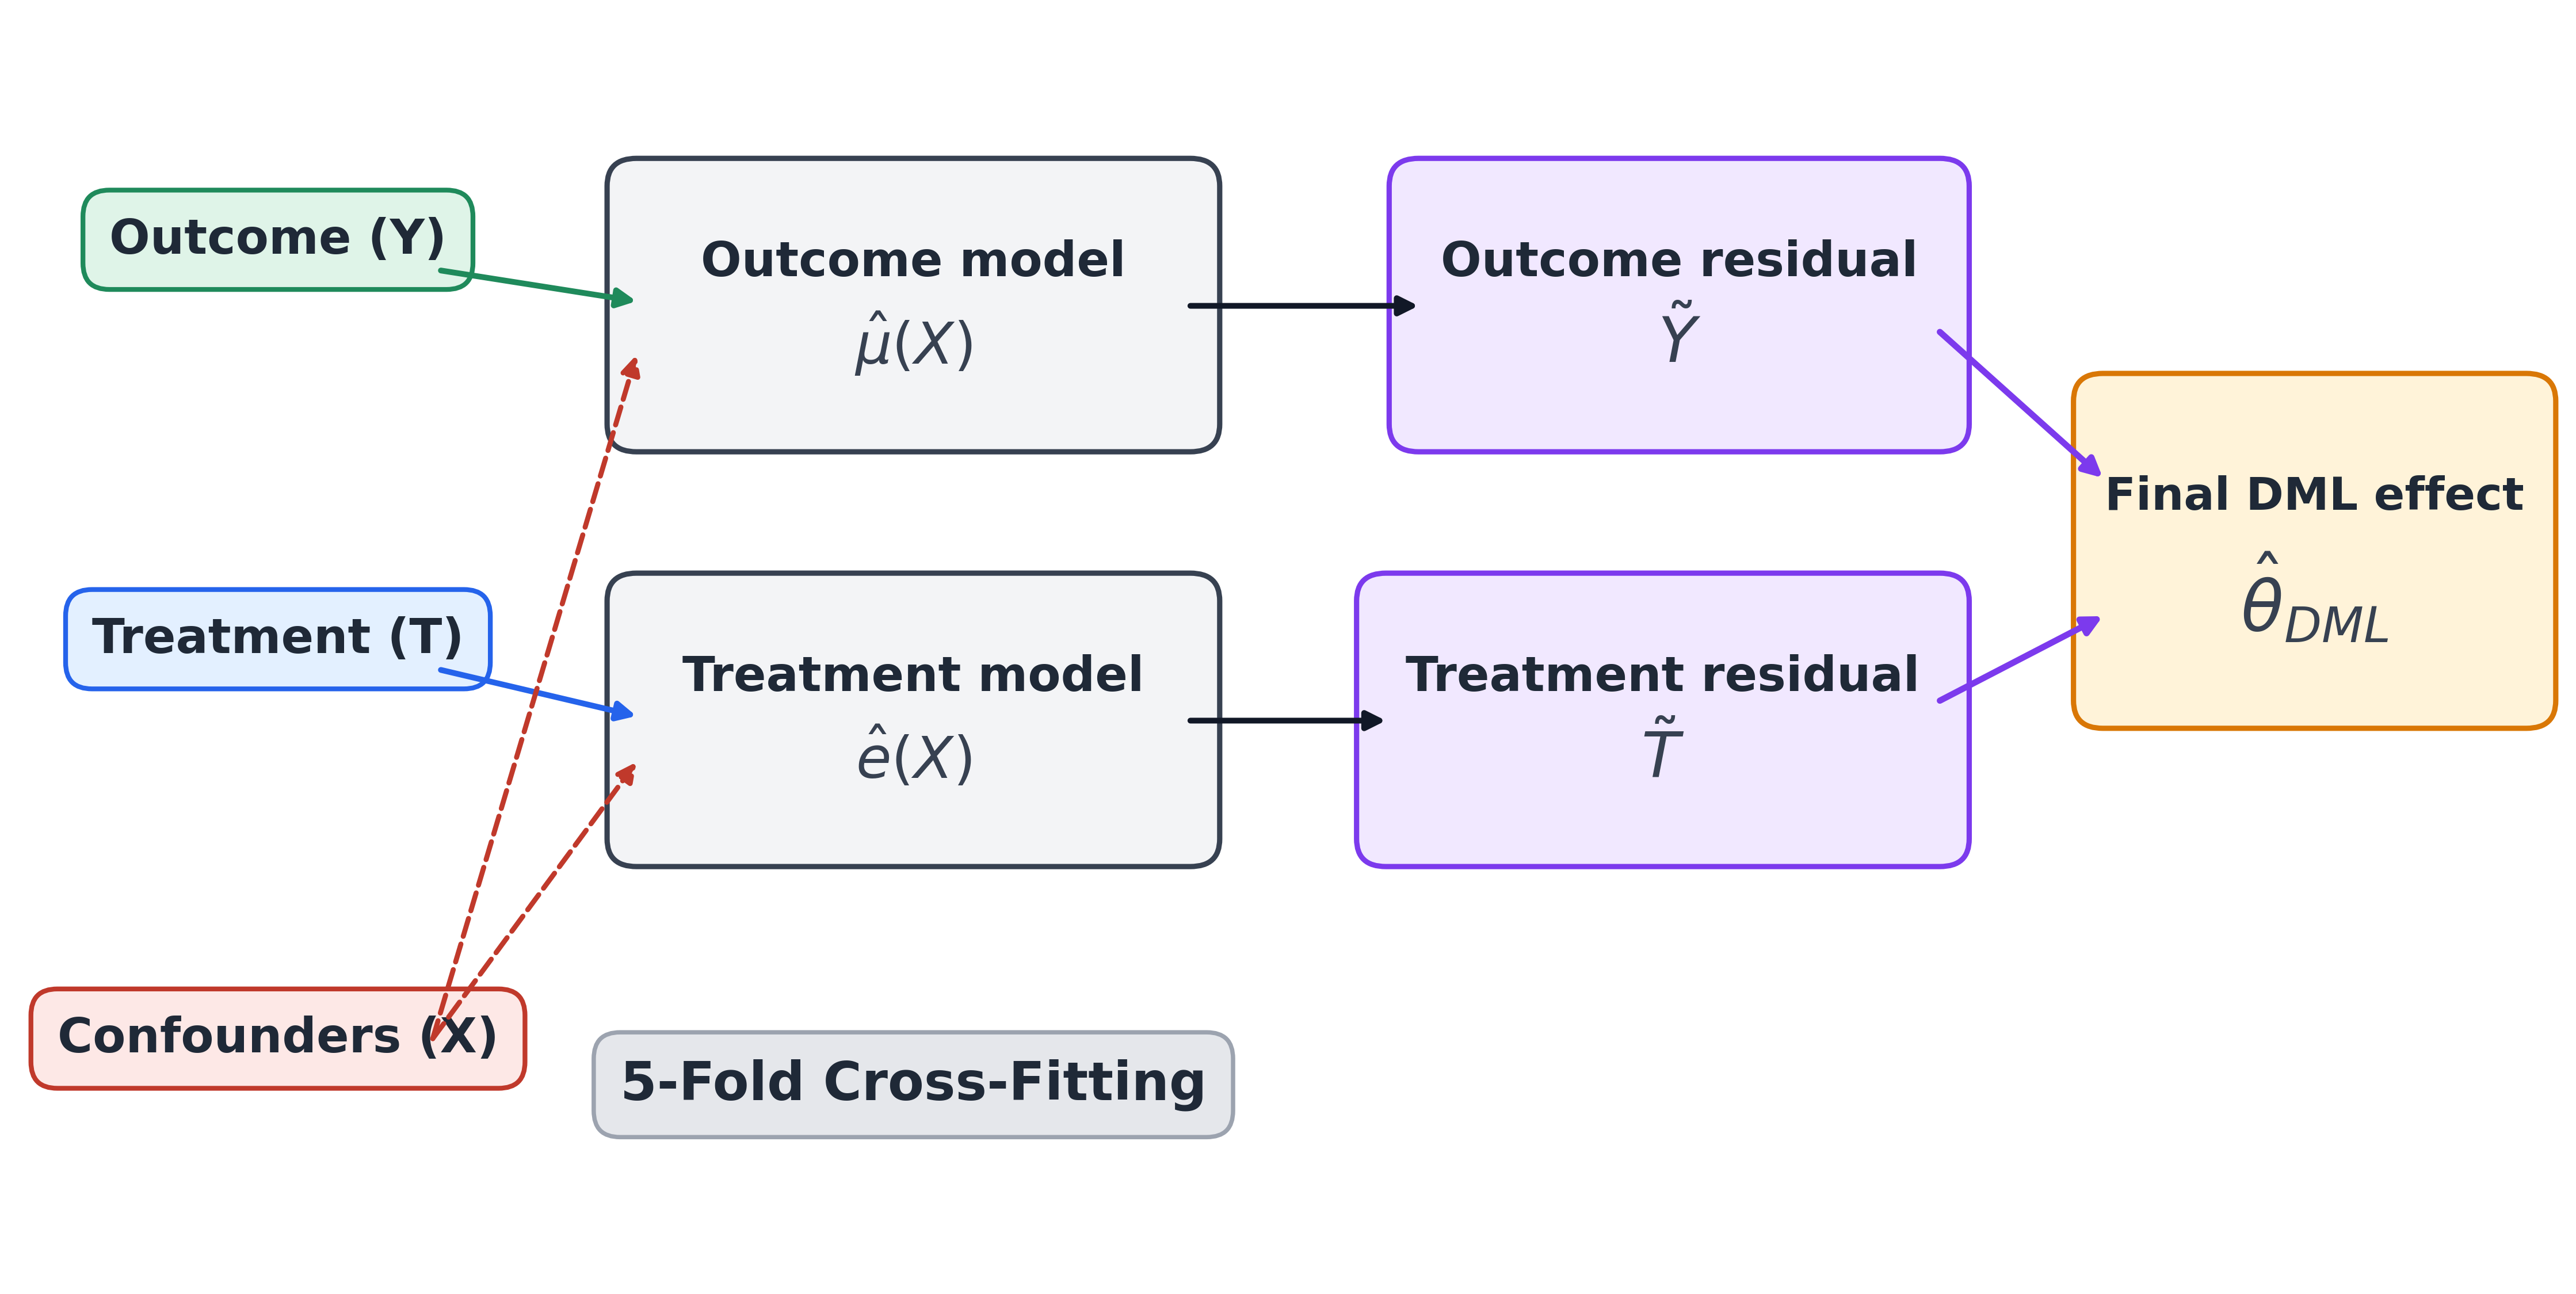
\includegraphics[width=1.04\textwidth]{figures/ch3/dml_schematic.png}}
\ownsource
\end{figure}

To reduce overfitting and regularization bias in nuisance estimation, the data is split into 5 folds ($K=5$) for cross-fitting. This ensures that residuals are always generated using models trained on out-of-sample data.

The estimation follows the DML orthogonalization and inference framework introduced by \citeA{chernozhukov2018double} and implemented using the LinearDML estimator from the econml Python library \cite{econml}. The nuisance models utilize Random Forest \cite{breiman2001random} specifications whose complexity is scaled proportionally to the sample size of each estimator. To prevent overfitting in the smaller stratified subsamples, the model capacity is regularized using a shallower maximum tree depth of 8 and 100 estimators, whereas a deeper architecture (maximum depth of 15, 200 estimators) is utilized for the full-sample estimator to capture more intricate non-linear confounder interactions.

The cross-validated $R^2$ scores of the nuisance models are used as a practical check of model behavior. If the treatment model achieved an extremely high $R^2$, it would suggest that the observed confounders almost fully determine treatment intensity, leaving little independent variation for effect estimation. Lower treatment predictability is therefore preferable in this setting.

Multicollinearity among the continuous treatment variables was checked using the variance inflation factor (VIF):
\begin{equation}
\mathrm{VIF}_k = \frac{1}{1 - R_k^2}
\end{equation}
Here, $k$ indexes a treatment variable, and $R_k^2$ is obtained by regressing treatment variable $k$ on the remaining treatment variables. Following \cite{obrien2007}, VIF values are treated as contextual diagnostics rather than fixed pass-or-fail thresholds.

Finally, because unmeasured confounding cannot be ruled out mechanically, estimates that are statistically significant at the 5\% level are accompanied by E-value sensitivity diagnostics \cite{vanderweele2017sensitivity}. These values are used only as approximate sensitivity checks for unmeasured confounding. They contribute to the interpretation by showing how strong an omitted factor would need to be to explain away the significant DML estimates.

To determine the average marginal effect of each signal characteristic, the model analyzes all three treatment variables simultaneously by regressing the outcome residuals directly onto the treatment residuals (Equation~\eqref{eq:final_causal_effect}). This simultaneous estimation estimates the association for each characteristic, such as \textit{Hype Intensity}, while adjusting for the other signal features included in the treatment vector.

Because the implemented specification uses ensemble nuisance models, statistical uncertainty is summarized with bootstrap-based inference. Bootstrapping repeatedly draws random samples with replacement from the original dataset and refits the estimator on each resampled dataset. In the implemented specification, the DML procedure is paired with the BootstrapInference module from the econml Python library using 500 iterations. Confidence intervals are constructed from the empirical distribution of the bootstrap estimates and are used to summarize coefficient precision in the reported results.

\section{Market-Cap Heterogeneity and Predictive Modeling}
\label{sec:stratified-estimation}
\label{sec:causal-forests}
\label{sec:predictive-modeling}

A single average effect can hide significant differences between coins of various sizes. Because highly liquid markets naturally resist simple manipulation, the causal estimation is performed separately across the four \textit{Market Capitalization} strata reported in Table~\ref{tab:sample-distribution}.
Running the DML pipeline independently across these segments ensures that extreme volatility from tiny micro-cap coins does not artificially contaminate the effect estimates for the more stable mid and large cap coins.
Together with the CATE (Conditional Average Treatment Effect) analysis below, this design tests the second hypothesis by asking whether market size changes the estimated signal effects.

Dividing coins into broad market-cap buckets can hide useful continuous information. To understand exactly how \textit{Market Capitalization} ($M_i$) influences the marginal response to each signal feature, the CATE is defined as the conditional average marginal treatment effect, following the EconML continuous-treatment formulation \cite{econml}:
\begin{equation}
\tau_j(m) = \frac{\partial}{\partial t_j}\mathbb{E}[Y_i(\mathbf{t}) \mid M_i = m]
\label{eq:cate}
\end{equation}
Here, $j$ indexes a treatment feature, $t_j$ is the value of that feature, and $m$ is a specific market-cap level.

To map these localized treatment effects, a Causal Forest is used \cite{athey2019generalized,econml}. Unlike standard Random Forests, which split data to group observations with similar outcomes, Causal Forests split the data to recover heterogeneity in treatment response. Across the ensemble, observations that frequently share leaves receive higher adaptive weights, and these forest-aggregated local weights are used to estimate observation-specific local Conditional Average Treatment Effects \cite{athey2019generalized,econml}.

The Causal Forest incorporates an ensemble of 2,000 trees, requiring a minimum of 20 observations per leaf. Because the Causal Forest analyzes one treatment dimension at a time, the other two signal features are added to the control matrix for that specific loop. When one signal feature is analyzed as the treatment, the other two signal features are included as controls. The resulting estimate is therefore interpreted as the partial marginal response to that feature, conditional on the other signal characteristics and the pre-reveal confounders.

As a computational and regularization tradeoff, the underlying nuisance models inside the Causal Forest use smaller Random Forest structures capped at 100 trees and a maximum depth of 10. Ultimately, this modeling setup examines how an asset's vulnerability to manipulation evolves as its \textit{Market Capitalization} grows, showing where the impact of these organized signals begins to diminish.

The methodology then turns from causal estimation to a separate forecasting task.

The final phase treats pump outcome prediction as a binary classification task. The target variable has two classes: \textit{Success} for events with a strictly positive \textit{10-Minute Logarithmic Return}, and \textit{Non-Success} for events with a zero or negative return:
\begin{equation}
\mathrm{Success}_i =
\begin{cases}
1 & \text{if } Y_i > 0 \quad (\textit{Success}) \\
0 & \text{if } Y_i \le 0 \quad (\textit{Non-Success})
\end{cases}
\label{eq:success_definition}
\end{equation}
Here, $Y_i$ is the winsorized \textit{10-Minute Logarithmic Return} for pump event $i$ as defined in Equation~\eqref{eq:log-return}. A value of $1$ signifies a positive price response within the 10-minute post-reveal window, while $0$ represents a neutral or negative price movement.

The predictive modeling stage focuses on the relationship between observable pre-signal market variables and signal characteristics. Channel identity is excluded from this core analysis to reduce direct dependence on channel-specific histories and evaluate performance on previously unseen pump groups. XGBoost (Extreme Gradient Boosting), LightGBM, and Random Forest were tested as tree-based candidates, and Optuna (an automated tool for choosing suitable hyperparameters) was used to tune them inside the grouped training folds \cite{xgboost2016, lightgbm2017, breiman2001random, optuna2019}. Reported predictive performance is evaluated on a grouped 80/20 holdout split in which the test set contains only unseen channels. Chapter IV reports the selected \textit{Channel ID}-agnostic XGBoost model as the primary evidence, with secondary comparisons including \textit{Channel ID}. For the selected XGBoost model, feature importance is reported as a relative importance score. This score shows how strongly each variable helps the fitted model separate \textit{Success} from \textit{Non-Success} events. The values are useful for comparing predictors inside the same model, but they do not show causal effects.
